\section{Career Project Highlights}
\small{\textit{The following projects have significantly contributed to my experience as a maritime and coastal engineer:}}
\renewcommand{\topfraction}{.999}
\renewcommand{\floatpagefraction}{.999}%
\fboxsep=0pt%padding thickness
\fboxrule=0.5pt%border thickness

\FloatBarrier
\begin{table}[h!]
    \begin{tblr}{Q[halign=l,valign=h,wd=0.63\textwidth]Q[halign=r,valign=t]}
    {\entrytableprojecthighlight%
	{ESTDEF01PH01 AUKUS Submarine Rotational Force -- West}
	{2023 to Present}
	{}
	{Maritime Structures Lead for KBR}
	{Perth, Western Australia}
	{Client: Australian Department of Defence}
	{\vspace{1em}\begin{itemize}
		 \item From as early as 2027, AUKUS partners will have a rotational presence at HMAS \textit{Stirling} of UK and US nuclear-powered submarines -- known as 'Submarine Rotational Force-West'
		 \item Technical oversight of maritime structure infrastructure upgrades, including potential wharf strengthening work, new fender frames, dredging and associated small craft facilities. 
		 \item Underttaking nuclear safety related design process, including risk assessments, hazard identification and nuclear safety justification documentation.
		 \item Significant amounts of multi-disciplinary coordination due to the large amount of support services required to maintain the vessels.
		 \item Managed design to tight delivery schedule, given the commitments from the government and significant public interest in the project.
	 \end{itemize}}
	} & \fcolorbox{black}{black}{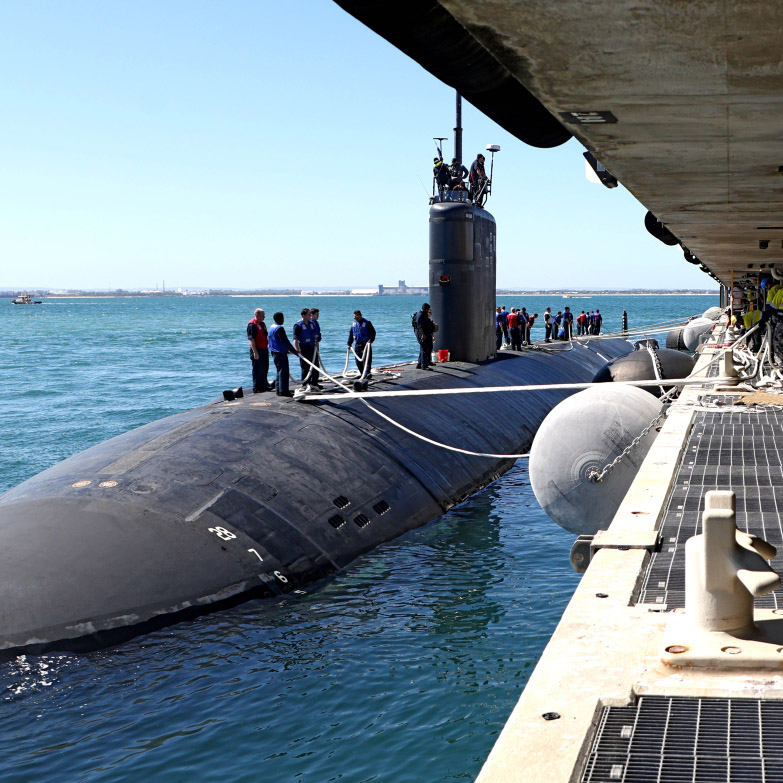
\includegraphics[width=6cm,height=6cm]{imgs/srf-w.jpg}} \\
    {\entrytableprojecthighlight%
	{SEA1180-1 NCIS-5 HMAS Coonawarra}
	{2023 to Present}
	{}
	{Maritime Design Lead for KBR}
	{Darwin, Northern Territory}
	{Client: Australian Department of Defence}
	{\vspace{1em}\begin{itemize}
		 \item Upgrade of existing wharf (including frontal pontoons) for homeporting of a number of new Arafura Class Offshore Patrol Vessels (ACOPVs).
		 \item Design solution required large frontal pontoons (to address Darwin's large tidal range) which were physically modelled to confirm behaviour in design events.
		 \item Technical oversight of maritime related construction support queries, including responding to RFIs, reviewing submittals and ensuring the Contractor met design intent.
		 \item Construction requires significant multi-disciplinary coordination due to the large amount of services required on the wharf.
		 \item Required to consider KBR's technical and commercial position when resolving issues arising on site.
	 \end{itemize}}
	} & \fcolorbox{black}{black}{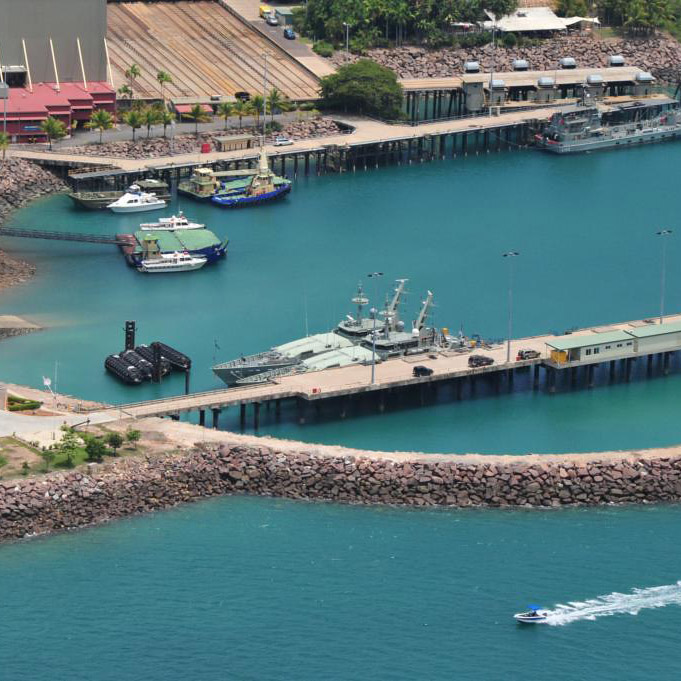
\includegraphics[width=6cm,height=6cm]{imgs/coonawarra.jpg}} \\
	{\entrytableprojecthighlight%
	{Australian Beach Erosion \& Coastal Flooding EWS}
	{2021 to 2023}
	{}
	{Research Associate for UNSW WRL}
	{Sydney, New South Wales}
	{}
	{\begin{itemize}
		\item Developed Early Warning System (EWS) for coastal storm hazards, publicly available \href{https://coastalews.wrl.unsw.edu.au/}{online} to deliver forecasts.
		\item System forecasts coastal flooding and beach erosion hazards across thousands of kilometres of shoreline across New South Wales and Western Australia.
		\item Responsible for developing methodology, models, data processing pipelines, automated workflows, and online dashboard.
		\item Gained an understanding of real-time forecasting systems over large areas, including scaling, monitoring and performance considerations.
		\item Liaised with and incorporated feedback from local, state and federal government project partners.
		\item Currently overseeing evaluation of system for to determine forecasting performance, with publication in preparation.
	 \end{itemize}}
	} & \fcolorbox{black}{black}{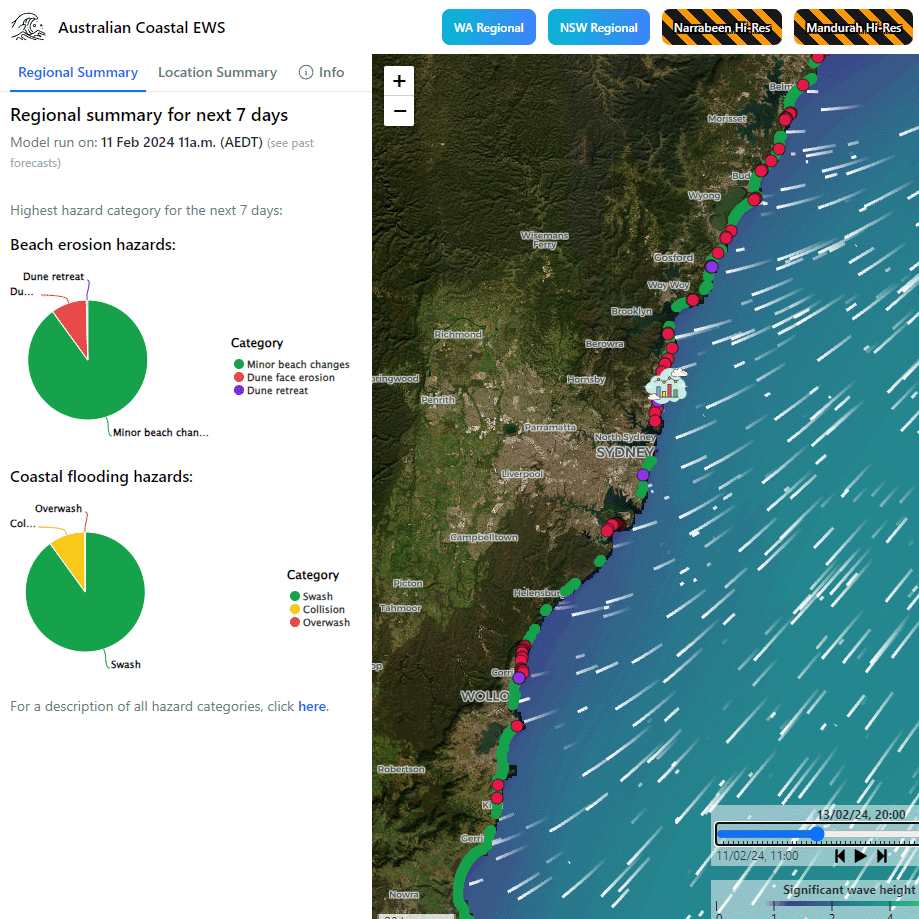
\includegraphics[width=6cm,height=6cm]{imgs/ews.png}} \\
	{\entrytableprojecthighlight%
	{Kingsford Smith Drive Upgrade}
	{2016 to 2018}
	{}
	{Maritime Structural Engineer for KBR}
	{Brisbane, Queensland}
	{Client: Lendlease and Brisbane City Council}
	{\vspace{1em}\begin{itemize}
		 \item Road widening along the Brisbane River, including a \SI{1.2}{\km} long marine retaining wall structure with cantilevered pedestrian and cycle path.
		 \item Responsibilities included performing detailed design calculations, writing design reports and specifications for the marine structure and associated works.
		 \item Design was required to consider a vessel impact design case, resulting in substantial loading onto the main structure and foundations.
		 \item Acquired substantial insitu and precast concrete detailing experience and was required to consider construction sequencing, creep, strut and tie design.
		 \item Designed a variety of smaller, miscellaneous structures, such as stone monument foundation, handrails, retaining walls, walkways and signs.  
		 \item Gained significant experience in a multi-disciplinary team, requiring coordination between roads, drainage, geotechnical, architectural, and electrical disciplines.
	 \end{itemize}}
	} & \fcolorbox{black}{black}{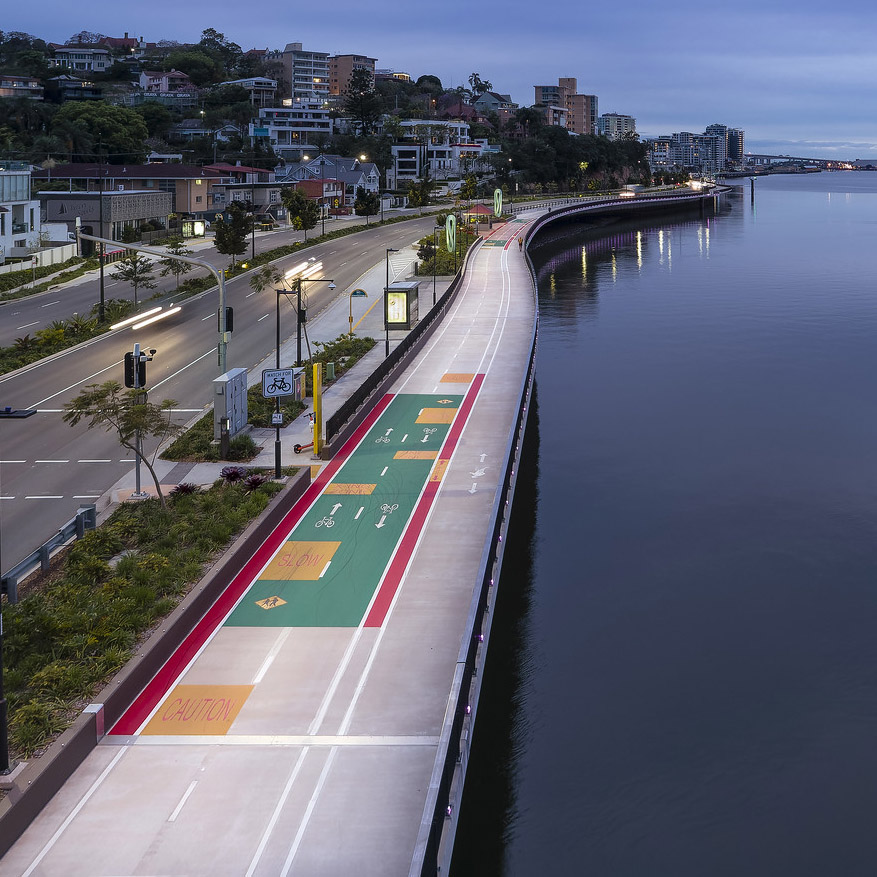
\includegraphics[width=6cm,height=6cm]{imgs/ksd.jpg}} \\
	% {\entrytableprojecthighlight%
	% {Townsville Port Inner Harbour Expansion (TPIX)}
	% {2012 to 2013}
	% {}
	% {Maritime Structural Engineer for KBR}
	% {Townsville, Queensland}
	% {Client: Port of Townsville}
	% {\begin{itemize}
	% 	 \item Reconstruction and extension of Berth 10 to accommodate military, cruise and commercial shipping, the construction of a new multi-purpose passenger terminal, and upgrade of Berth 8 to accommodate Panamax sized ships.
	% 	 \item Completing structural detailed design calculations for Berth 8 and Berth 10 works, developing design drawing and documentation.
	% 	 \item Performed on-site supervision of works on site. Required to consider KBR's technical and commerical position while resolving site issues.
	%  \end{itemize}}
	% } & \fcolorbox{black}{black}{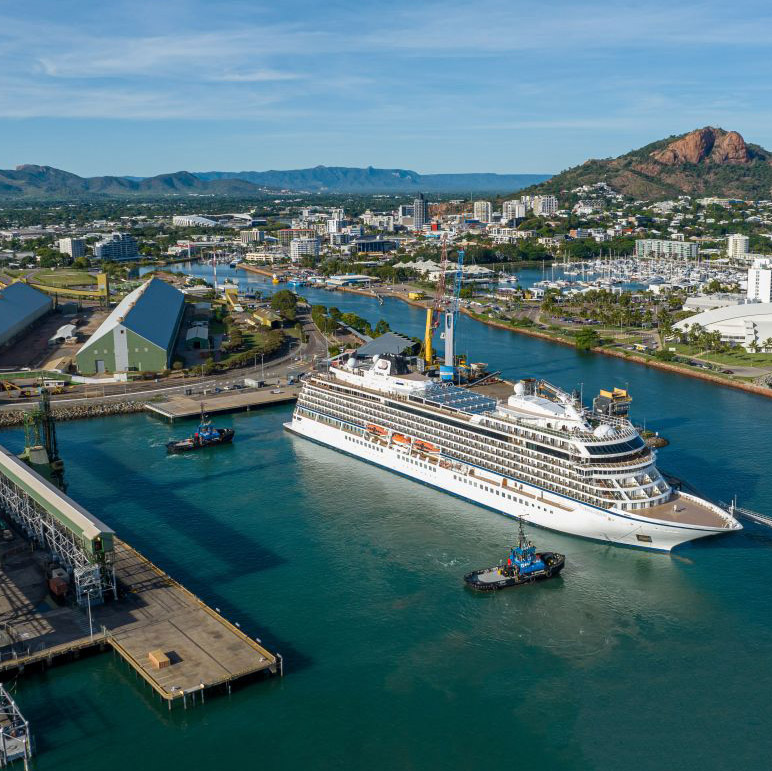
\includegraphics[width=6cm,height=6cm]{imgs/tpix.jpg}} \\
    \end{tblr}
\end{table}
\FloatBarrier
